%%
%% This is file `tikzposter-template.tex',
%% generated with the docstrip utility.
%%
%% The original source files were:
%%
%% tikzposter.dtx  (with options: `tikzposter-template.tex')
%%
%% This is a generated file.
%%
%% Copyright (C) 2014 by Pascal Richter, Elena Botoeva, Richard Barnard, and Dirk Surmann
%%
%% This file may be distributed and/or modified under the
%% conditions of the LaTeX Project Public License, either
%% version 2.0 of this license or (at your option) any later
%% version. The latest version of this license is in:
%%
%% http://www.latex-project.org/lppl.txt
%%
%% and version 2.0 or later is part of all distributions of
%% LaTeX version 2013/12/01 or later.
%%


\documentclass{tikzposter} %Options for format can be included here

\usepackage{todonotes}

\usepackage[tikz]{bclogo}
\usepackage{lipsum}
\usepackage{amsmath}

\usepackage{booktabs}
\usepackage{longtable}
\usepackage[absolute]{textpos}
\usepackage[it]{subfigure}
\usepackage{graphicx}
\usepackage{cmbright}
%\usepackage[default]{cantarell}
%\usepackage{avant}
%\usepackage[math]{iwona}
\usepackage[math]{kurier}
\usepackage[T1]{fontenc}


%% add your packages here
\usepackage{hyperref}
% for random text
\usepackage{lipsum}
\usepackage[english]{babel}
\usepackage[pangram]{blindtext}

\colorlet{backgroundcolor}{blue!10}

 % Title, Author, Institute
\title{Flip 01 Project Report}
\author{Baobao Song}
\institute{ Hunan University, China
}
%\titlegraphic{logos/tulip-logo.eps}

%Choose Layout
\usetheme{Wave}

%\definebackgroundstyle{samplebackgroundstyle}{
%\draw[inner sep=0pt, line width=0pt, color=red, fill=backgroundcolor!30!black]
%(bottomleft) rectangle (topright);
%}
%
%\colorlet{backgroundcolor}{blue!10}

\begin{document}


\colorlet{blocktitlebgcolor}{blue!23}

 % Title block with title, author, logo, etc.
\maketitle

\begin{columns}
 % FIRST column
\column{0.5}% Width set relative to text width

%%%%%%%%%% -------------------------------------------------------------------- %%%%%%%%%%
 %\block{Main Objectives}{
%  	      	\begin{enumerate}
%  	      	\item Formalise research problem by extending \emph{outlying aspects mining}
%  	      	\item Proposed \emph{GOAM} algorithm is to solve research problem
%  	      	\item Utilise pruning strategies to reduce time complexity
%  	      	\end{enumerate}
%%  	      \end{minipage}
%}
%%%%%%%%%% -------------------------------------------------------------------- %%%%%%%%%%


%%%%%%%%%% -------------------------------------------------------------------- %%%%%%%%%%
\block{Introduction}{
    This is a correlation prediction problem. Home Depot wants to improve their customers' shopping experience by developing a model that can accurately predict the relevance of search results of Home Depot product. Many information are given about product description and relevance ratings. And the goal is to predict the relevance for each pair that contains products and searches listed in the test set.The raw datasets contain five files, which attributes are shown below.
\bigskip     
		\vbox{}
   \begin{tabular}{cp{25cm}p{25cm}}
   	\hline
   	Name&Attribute\\
   	\hline
   	product\_descriptions.csv& product\_uid,product\_description\\
   	attributes.csv& product\_id,name,value\\
   	train.csv &id, product\_id, product\_title,search\_term, relevance\\
   	test.csv&id, product\_id, product\_title,search\_term\\
   	sample\_submission.csv&id,relevance\\
   	\hline
   \end{tabular}
}
%%%%%%%%%% -------------------------------------------------------------------- %%%%%%%%%%


%%%%%%%%%% -------------------------------------------------------------------- %%%%%%%%%%
\block{Test Preprocessing}{
\begin{itemize}
    \item Merge test.csv and train.csv datasets and concat  product description(product\_descriptions),name and value(attributes.csv)
    \item Convert to lowercase
    \item Remove punctuation
    \item Remove stopwords
    \item Stemming by SnowballStemmer
\end{itemize}
}
%%%%%%%%%% -------------------------------------------------------------------- %%%%%%%%%%


%%%%%%%%%% -------------------------------------------------------------------- %%%%%%%%%%

%\note{Note with default behavior}

%\note[targetoffsetx=12cm, targetoffsety=-1cm, angle=20, rotate=25]
%{Note \\ offset and rotated}

 % First column - second block


%%%%%%%%%% -------------------------------------------------------------------- %%%%%%%%%%
\block{Text features}{
\begin{itemize}
    \item Fundamental feature1:the length of search term
    \item Fundamental feature2:the number of same keywords between search terms and product title
    \item Fundamental feature3:the number of same keywords between search terms and product description
    \item Levenshtein feature1:Levenshtein text similarity between search terms and product title
    \item Levenshtein feature2:Levenshtein text similarity between search terms and product description
    \item TF-IDF feature1:Cosine similarity between search terms and product title
    \item TF-IDF feature2:Cosine similarity between search terms and product description
    \item Word2Vec feature1:Cosine similarity between search terms and product title
	\item Word2Vec feature2:Cosine similarity between search terms and product description
\end{itemize}
}
%%%%%%%%%% -------------------------------------------------------------------- %%%%%%%%%%


% SECOND column
\column{0.5}
 %Second column with first block's top edge aligned with with previous column's top.

%%%%%%%%%% -------------------------------------------------------------------- %%%%%%%%%%
\block{Different Models and Parameters Adjustment}{
	Using different models to predict the relevance and choose the best one. In each method, adjusting parameters include max
	depth and iterations. CV error is used to judge the model performance and its scoring is MSE. The models and the process of parameters adjustment(such as g max depth of Gradient Boosting Regressor) are below.
	
\begin{itemize}
	\item Bagging Regression
	\item Gradient Boost Regression
	\item Random Forest Regression
	\item XGB Regression 
\end{itemize}

\begin{tikzfigure}%[Overall architecture of \emph{GOAM} algorithm]
    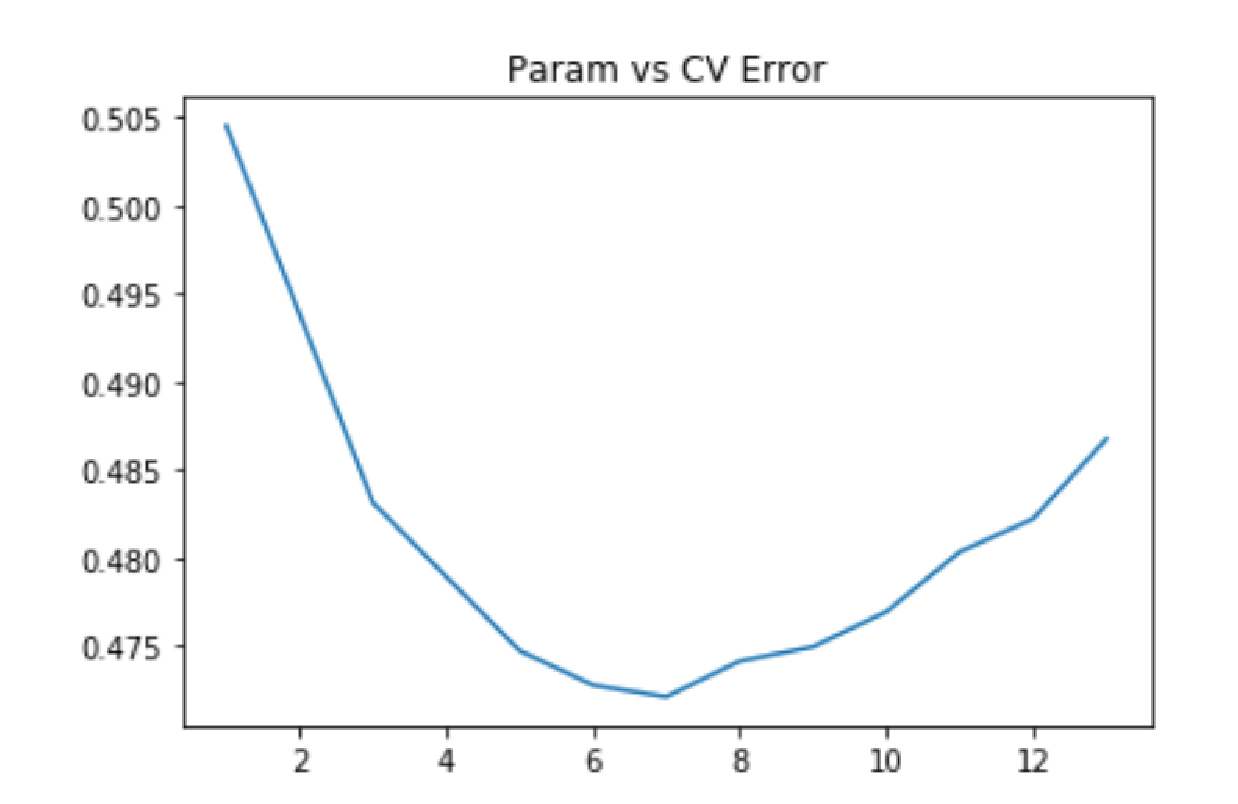
\includegraphics[width=30cm, height=17cm]{figures/adjust3.eps}
\end{tikzfigure}
 
}
%%%%%%%%%% -------------------------------------------------------------------- %%%%%%%%%%
% Second column - first block


%%%%%%%%%% -------------------------------------------------------------------- %%%%%%%%%%
\block[titleleft]{Results}
{
\begin{itemize}
	\item Model performance:Gradient Boost Regression>Random Forest Regression>XGB Regression>Bagging Regression
	\item Parameter(Gradient Boost Regression):max\_depth:7,iteration:30
	\item Score:0.47101(RMSE)
	\item Rank:347/2123
\end{itemize}
}
%%%%%%%%%% -------------------------------------------------------------------- %%%%%%%%%%


% Second column - second block
%%%%%%%%%% -------------------------------------------------------------------- %%%%%%%%%%
\block[titlewidthscale=1, bodywidthscale=1]
{Conclusion}
{
 Compare to midterm presentation, MSE decreased from 0.48032 to 0.4710. The reason mainly is more features and different modeling. Different features that use different method can help the final model predict well. And by adjusting four models' parameters, Gradient Boost Regression perform best. In the next step, using more information about product and fine-tuned parameters may lead a better result. 

}
%%%%%%%%%% -------------------------------------------------------------------- %%%%%%%%%%


% Bottomblock
%%%%%%%%%% -------------------------------------------------------------------- %%%%%%%%%%

%\note[targetoffsetx=8cm, targetoffsety=-10cm,rotate=0,angle=180,radius=8cm,width=.46\textwidth,innersep=.1cm]{
%Acknowledgement
%}

%\block[titlewidthscale=0.9, bodywidthscale=0.9]
%{Acknowledgement}{
%}
%%%%%%%%%% -------------------------------------------------------------------- %%%%%%%%%%

\end{columns}


%%%%%%%%%% -------------------------------------------------------------------- %%%%%%%%%%
%[titleleft, titleoffsetx=2em, titleoffsety=1em, bodyoffsetx=2em,%
%roundedcorners=10, linewidth=0mm, titlewidthscale=0.7,%
%bodywidthscale=0.9, titlecenter]

%\colorlet{noteframecolor}{blue!20}
\colorlet{notebgcolor}{blue!20}
\colorlet{notefrcolor}{blue!20}
\note[targetoffsetx=-13cm, targetoffsety=-12cm,rotate=0,angle=180,radius=8cm,width=.96\textwidth,innersep=.4cm]
{
\begin{minipage}{0.3\linewidth}
\centering

\includegraphics[width=24cm]{logos/tulip-wordmark.eps}
\end{minipage}
\begin{minipage}{0.7\linewidth}
{ \centering
 Flip01 project report,01/15/2021,changsha,China
}
\end{minipage}
}
%%%%%%%%%% -------------------------------------------------------------------- %%%%%%%%%%


\end{document}

%\endinput
%%
%% End of file `tikzposter-template.tex'.
